\documentclass[aspectratio=169,10pt]{beamer}

\usetheme{Copenhagen}
\usecolortheme{dolphin}
\usefonttheme{professionalfonts}

\usepackage[T1]{fontenc}
\usepackage{lmodern}
\usepackage{amsmath}
\usepackage{booktabs}
\usepackage{listings}
\usepackage{tikz}
\usepackage{array}
\usepackage{ragged2e}
\usepackage{hyperref}

\definecolor{SGBlue}{RGB}{0,82,155}
\definecolor{SGNavy}{RGB}{0,45,90}
\definecolor{SGLightBlue}{RGB}{232,242,252}
\definecolor{SGMidBlue}{RGB}{90,150,210}
\definecolor{SGGray}{RGB}{70,78,88}
\definecolor{SGCodeBg}{RGB}{246,249,253}

\setbeamercolor{structure}{fg=SGBlue}
\setbeamercolor{palette primary}{fg=white,bg=SGBlue}
\setbeamercolor{palette secondary}{fg=white,bg=SGNavy}
\setbeamercolor{palette tertiary}{fg=white,bg=SGBlue!75!black}
\setbeamercolor{frametitle}{fg=SGNavy}
\setbeamercolor{title}{fg=SGNavy}
\setbeamercolor{author}{fg=SGGray}
\setbeamercolor{institute}{fg=SGGray}
\setbeamercolor{date}{fg=SGGray}
\setbeamercolor{block title}{fg=white,bg=SGBlue}
\setbeamercolor{block body}{fg=black,bg=SGLightBlue}
\setbeamercolor{alerted text}{fg=SGBlue!80!black}
\setbeamercolor{normal text}{fg=black,bg=white}
\setbeamertemplate{navigation symbols}{}
\setbeamertemplate{itemize item}{\color{SGBlue}$\blacktriangleright$}
\setbeamertemplate{itemize subitem}{\color{SGMidBlue}$\bullet$}
\setbeamertemplate{footline}{%
  \leavevmode%
  \hbox{%
    \begin{beamercolorbox}[wd=.82\paperwidth,ht=2.5ex,dp=.8ex,leftskip=1em]{author in head/foot}%
      \usebeamerfont{author in head/foot}\insertshorttitle
    \end{beamercolorbox}%
    \begin{beamercolorbox}[wd=.18\paperwidth,ht=2.5ex,dp=.8ex,rightskip=1em plus 1fil]{date in head/foot}%
      \usebeamerfont{date in head/foot}\hfill\insertframenumber{} / \inserttotalframenumber
    \end{beamercolorbox}%
  }%
}

\lstdefinestyle{go}{
  language=Go,
  basicstyle=\ttfamily\scriptsize,
  keywordstyle=\color{SGBlue}\bfseries,
  commentstyle=\color{SGGray}\itshape,
  stringstyle=\color{green!45!black},
  backgroundcolor=\color{SGCodeBg},
  frame=single,
  rulecolor=\color{SGMidBlue!45},
  framerule=.5pt,
  showstringspaces=false,
  columns=fullflexible,
  keepspaces=true,
  breaklines=true,
  tabsize=2
}
\lstdefinestyle{wire}{
  basicstyle=\ttfamily\small,
  backgroundcolor=\color{SGCodeBg},
  frame=single,
  rulecolor=\color{SGMidBlue!45},
  showstringspaces=false,
  columns=fullflexible,
  keepspaces=true,
  breaklines=true
}
\lstset{style=go}

\newcommand{\blue}[1]{\textcolor{SGBlue}{#1}}
\newcommand{\code}[1]{\texttt{\small #1}}
\newcommand{\good}[1]{\textcolor{green!45!black}{#1}}
\newcommand{\warn}[1]{\textcolor{orange!80!black}{#1}}

\title[Socket-Go Protocol]{Socket-Go Messaging Protocol}
\subtitle{Design, Application-Layer Semantics, and Implementation}
\author{Suphachock Kamlek -- 6710451321}
\institute{Computer Communications \/ Computer Science}
\date{\today}

\begin{document}

\begin{frame}
  \titlepage
\end{frame}

\begin{frame}{Presentation roadmap}
  \begin{enumerate}
    \item Purpose and requirements
    \item Protocol design and wire format
    \item Runtime semantics: publish, delivery, ACK, and retry
    \item Implementation walkthrough
    \item Testing and performance evaluation
    \item Limitations, future work, and final architecture
  \end{enumerate}
\end{frame}

\section{Purpose and Requirements}

\begin{frame}{The problem: reliable messaging over a byte stream}
  \begin{columns}[T,onlytextwidth]
    \column{.48\textwidth}
      \begin{block}{What the application needs}
        \begin{itemize}
          \item Route messages by topic.
          \item Support independent publishers and consumers.
          \item Deliver asynchronously over long-lived connections.
          \item Detect processing success with application-level ACK.
          \item Recover from slow consumers and lost sessions.
        \end{itemize}
      \end{block}
    \column{.48\textwidth}
      \begin{block}{Why TCP alone is not enough}
        \begin{itemize}
          \item TCP transports an ordered byte stream, not messages.
          \item A successful TCP write is not a successful business operation.
          \item The server still needs framing, routing, ACK, and retry rules.
        \end{itemize}
      \end{block}
  \end{columns}
\end{frame}

\begin{frame}{Program objective}
  \begin{block}{Application definition}
    Socket-Go is a topic-based messaging broker implemented as a custom
    application-layer protocol over TCP.
  \end{block}
  \vspace{.35em}
  \begin{columns}[T,onlytextwidth]
    \column{.32\textwidth}
      \centering\blue{Publisher}\\[.35em]
      \small Sends a message to a topic.
    \column{.34\textwidth}
      \centering\blue{Broker}\\[.35em]
      \small Queues and routes messages.
    \column{.32\textwidth}
      \centering\blue{Consumer}\\[.35em]
      \small Receives and acknowledges work.
  \end{columns}
  \vspace{.8em}
  \begin{center}
    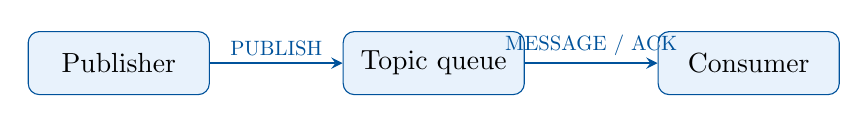
\begin{tikzpicture}[>=stealth]
      \node[draw=SGBlue,fill=SGLightBlue,rounded corners,minimum width=2.3cm,minimum height=.8cm] (p) at (0,0) {Publisher};
      \node[draw=SGBlue,fill=SGLightBlue,rounded corners,minimum width=2.3cm,minimum height=.8cm] (t) at (4,0) {Topic queue};
      \node[draw=SGBlue,fill=SGLightBlue,rounded corners,minimum width=2.3cm,minimum height=.8cm] (c) at (8,0) {Consumer};
      \draw[->,thick,SGBlue] (p) -- node[above,sloped,scale=.75]{PUBLISH} (t);
      \draw[->,thick,SGBlue] (t) -- node[above,sloped,scale=.75]{MESSAGE / ACK} (c);
    \end{tikzpicture}
  \end{center}
\end{frame}

\begin{frame}{Application characteristics}
  \begin{itemize}
    \item \textbf{Asynchronous:} the publisher does not wait for consumer processing.
    \item \textbf{Topic-based:} routing is determined by a logical topic name.
    \item \textbf{Multiplexed:} several logical channels share one TCP connection.
    \item \textbf{At-least-once:} missing ACKs may cause redelivery.
    \item \textbf{Backpressure-aware:} pending queue and in-flight limits are bounded.
    \item \textbf{Concurrent:} sessions, Exchange, and Topics run independently.
    \item \textbf{Actor-owned state:} Exchange/Topic serialize state through commands.
  \end{itemize}
  \vspace{.45em}
  \begin{alertblock}{Important consequence}
    Consumers must tolerate duplicate \code{MessageID} values and should perform
    application-level deduplication when the operation is not idempotent.
  \end{alertblock}
\end{frame}

\begin{frame}{Why TCP instead of UDP?}
  \small
  \begin{tabular}{>{\raggedright\arraybackslash}p{.32\textwidth}cc}
    \toprule
    Requirement & TCP & UDP \\
    \midrule
    Ordered byte stream & \good{Yes} & \warn{No} \\
    Retransmission & \good{Built in} & \warn{Application must implement} \\
    Flow / congestion control & \good{Built in} & \warn{Not provided} \\
    Long-lived full-duplex session & \good{Natural} & Possible, but custom \\
    Message-level ACK & \warn{Still needed} & \warn{Still needed} \\
    \bottomrule
  \end{tabular}
  \vspace{.55em}
  \begin{block}{Decision}
    Use TCP for transport reliability, then add application semantics for
    framing, processing acknowledgement, retry, and routing.
  \end{block}
\end{frame}

\section{Protocol Design}

\begin{frame}{Layered design}
  \begin{center}
    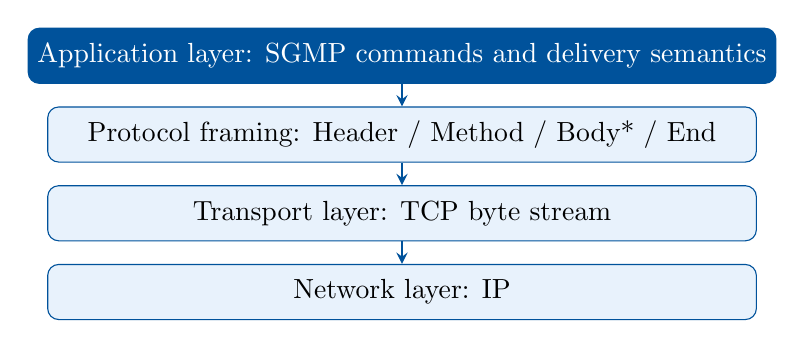
\begin{tikzpicture}[>=stealth]
      \node[draw=SGBlue,fill=SGBlue,text=white,rounded corners,minimum width=9cm,minimum height=.7cm] (app) at (0,2.1) {Application layer: SGMP commands and delivery semantics};
      \node[draw=SGBlue,fill=SGLightBlue,rounded corners,minimum width=9cm,minimum height=.7cm] (frame) at (0,1.1) {Protocol framing: Header / Method / Body* / End};
      \node[draw=SGBlue,fill=SGLightBlue,rounded corners,minimum width=9cm,minimum height=.7cm] (tcp) at (0,.1) {Transport layer: TCP byte stream};
      \node[draw=SGBlue,fill=SGLightBlue,rounded corners,minimum width=9cm,minimum height=.7cm] (ip) at (0,-.9) {Network layer: IP};
      \draw[->,thick,SGBlue] (app) -- (frame);
      \draw[->,thick,SGBlue] (frame) -- (tcp);
      \draw[->,thick,SGBlue] (tcp) -- (ip);
    \end{tikzpicture}
  \end{center}
  \vspace{.35em}
  \begin{itemize}
    \item TCP provides transport, not application messages.
    \item Framing makes message boundaries explicit.
    \item The application layer defines observable behavior and guarantees.
  \end{itemize}
\end{frame}

\begin{frame}{Wire format: one frame}
  \begin{center}
    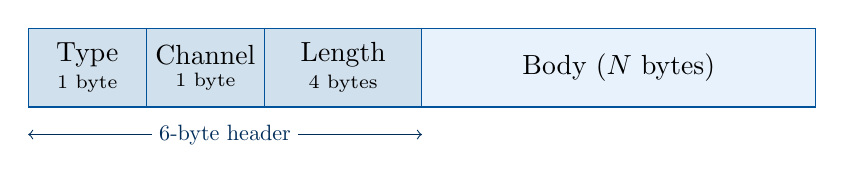
\begin{tikzpicture}[x=1cm,y=1cm]
      \draw[fill=SGBlue!18,draw=SGBlue] (0,0) rectangle (1.5,1);
      \draw[fill=SGBlue!18,draw=SGBlue] (1.5,0) rectangle (3,1);
      \draw[fill=SGBlue!18,draw=SGBlue] (3,0) rectangle (5,1);
      \draw[fill=SGLightBlue,draw=SGBlue] (5,0) rectangle (10,1);
      \node at (.75,.5) {\shortstack{Type\\\scriptsize 1 byte}};
      \node at (2.25,.5) {\shortstack{Channel\\\scriptsize 1 byte}};
      \node at (4,.5) {\shortstack{Length\\\scriptsize 4 bytes}};
      \node at (7.5,.5) {Body ($N$ bytes)};
      \draw[<->,SGNavy] (0,-.35) -- node[fill=white,scale=.8]{6-byte header} (5,-.35);
    \end{tikzpicture}
  \end{center}
  \vspace{.6em}
  \begin{itemize}
    \item Integer fields use network byte order (big-endian).
    \item A frame body is limited to 1024 bytes.
    \item Larger logical payloads use multiple Body frames.
  \end{itemize}
\end{frame}

\begin{frame}[fragile]{Wire format: frame types}
  \begin{columns}[T,onlytextwidth]
    \column{.47\textwidth}
    \begin{lstlisting}[style=wire]
0  Header      key=value metadata
1  Method      PUBLISH, ACK, PING, ...
2  Body        payload fragment
3  Heartbeat   standalone liveness frame
4  End         logical message terminator
    \end{lstlisting}
    \column{.49\textwidth}
    \begin{block}{Logical message grammar}
      \centering
      \code{Header Method Body* End}
    \end{block}
    \begin{itemize}
      \item Every frame in one logical message uses the same channel.
      \item The processor rejects invalid order or channel mismatch.
      \item Heartbeat is the only standalone frame sequence.
    \end{itemize}
  \end{columns}
\end{frame}

\begin{frame}[fragile]{Logical channels are not Go channels}
  \begin{columns}[T,onlytextwidth]
    \column{.46\textwidth}
    \begin{block}{Protocol meaning}
      A channel is a logical stream multiplexed inside one TCP connection.
    \end{block}
    \begin{itemize}
      \item Channel ID is carried in every frame.
      \item The server associates a channel with one session.
      \item A channel has a role: publisher or consumer.
    \end{itemize}
    \column{.48\textwidth}
    \begin{lstlisting}[style=wire]
TCP connection
  channel 1: consumer / control
  channel 2: publisher

SUBSCRIBE -> ConsumerChannel
PUBLISH   -> PublisherChannel
MESSAGE   -> ConsumerChannel
ACK       -> ConsumerChannel
    \end{lstlisting}
  \end{columns}
  \vspace{.3em}
  \begin{alertblock}{Protocol rule}
    A channel MUST NOT change role after it has been established.
  \end{alertblock}
\end{frame}

\begin{frame}{Command model}
  \small
  \begin{tabular}{>{\ttfamily}p{.22\textwidth}p{.28\textwidth}p{.38\textwidth}}
    \toprule
    Command & Direction & Meaning \\
    \midrule
    PUBLISH & Client $\rightarrow$ Server & Append a message to a topic queue \\
    SUBSCRIBE & Client $\rightarrow$ Server & Register a consumer channel \\
    UNSUBSCRIBE & Client $\rightarrow$ Server & Remove a topic subscription \\
    MESSAGE & Server $\rightarrow$ Client & Deliver one message \\
    ACK & Client $\rightarrow$ Server & Confirm successful processing \\
    NACK & Client $\rightarrow$ Server & Reject and requeue a delivery \\
    TOPICS & Client $\rightarrow$ Server & Query topic names \\
    PING / PONG & Both directions & Liveness check \\
    EXIT / BYE & Both directions & Graceful connection close \\
    \bottomrule
  \end{tabular}
\end{frame}

\begin{frame}{Message identity and delivery identity}
  \begin{columns}[T,onlytextwidth]
    \column{.48\textwidth}
      \begin{block}{Message identity}
        \begin{itemize}
          \item \code{MessageID} identifies the original message.
          \item It remains unchanged across retries.
          \item It is the key for consumer deduplication.
        \end{itemize}
      \end{block}
    \column{.48\textwidth}
      \begin{block}{Delivery identity}
        \begin{itemize}
          \item \code{DeliveryID} identifies one delivery attempt.
          \item It is the identifier carried by ACK/NACK.
          \item A retry creates a new DeliveryID.
        \end{itemize}
      \end{block}
  \end{columns}
  \vspace{.5em}
  \begin{center}
    \code{MessageID = M1} \quad $\Rightarrow$ \quad
    \code{DeliveryID = D1, attempt=1} \quad $\Rightarrow$ \quad
    \code{DeliveryID = D2, attempt=2}
  \end{center}
\end{frame}

\section{Runtime Semantics}

\begin{frame}{Publish path}
  \begin{enumerate}
    \item The client sends \code{PUBLISH} on a PublisherChannel.
    \item Session and FrameProcessor assemble one \code{FullFrame}.
    \item Process validates channel ownership and message size.
    \item Exchange resolves the topic.
    \item Topic appends the message to its bounded pending queue.
    \item The server returns \code{PUBLISH\_OK} after queue acceptance.
  \end{enumerate}
  \vspace{.5em}
  \begin{alertblock}{Meaning of PUBLISH\_OK}
    The broker accepted the message; it does not mean that a consumer has
    finished processing it.
  \end{alertblock}
\end{frame}

\begin{frame}{Delivery path}
  \begin{center}
    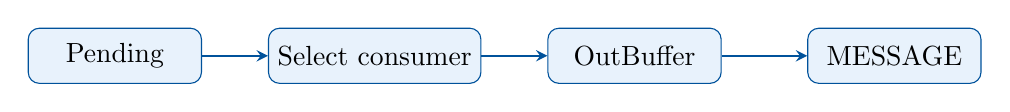
\begin{tikzpicture}[>=stealth]
      \node[draw=SGBlue,fill=SGLightBlue,rounded corners,minimum width=2.2cm,minimum height=.7cm] (p) at (0,0) {Pending};
      \node[draw=SGBlue,fill=SGLightBlue,rounded corners,minimum width=2.2cm,minimum height=.7cm] (s) at (3.3,0) {Select consumer};
      \node[draw=SGBlue,fill=SGLightBlue,rounded corners,minimum width=2.2cm,minimum height=.7cm] (o) at (6.6,0) {OutBuffer};
      \node[draw=SGBlue,fill=SGLightBlue,rounded corners,minimum width=2.2cm,minimum height=.7cm] (m) at (9.9,0) {MESSAGE};
      \draw[->,thick,SGBlue] (p) -- (s);
      \draw[->,thick,SGBlue] (s) -- (o);
      \draw[->,thick,SGBlue] (o) -- (m);
    \end{tikzpicture}
  \end{center}
  \vspace{.6em}
  \begin{itemize}
    \item Topic chooses an eligible consumer using round-robin order.
    \item The delivery is inserted into \code{unacked} before further progress.
    \item A consumer receives \code{MESSAGE} and ACKs after processing.
  \end{itemize}
\end{frame}

\begin{frame}{ACK, NACK, timeout, and retry}
  \begin{columns}[T,onlytextwidth]
    \column{.48\textwidth}
      \begin{block}{ACK}
        \begin{itemize}
          \item Validate channel ownership.
          \item Remove DeliveryID from \code{unacked}.
          \item Decrease in-flight count.
          \item Release capacity for the next message.
        \end{itemize}
      \end{block}
    \column{.48\textwidth}
      \begin{block}{NACK / timeout}
        \begin{itemize}
          \item Remove the old delivery.
          \item Requeue the same MessageID.
          \item Increment attempt and create a new DeliveryID.
          \item Drop after the retry limit is reached.
        \end{itemize}
      \end{block}
  \end{columns}
  \vspace{.45em}
  \begin{center}
    \code{pending $\rightarrow$ unacked $\rightarrow$ ACK} \qquad
    \code{pending $\leftarrow$ timeout / NACK}
  \end{center}
\end{frame}

\begin{frame}[fragile]{Backpressure and max in-flight}
  \begin{block}{Definition}
    \code{maxInFlight} is the maximum number of deliveries sent to one
    consumer that have not received ACK yet.
  \end{block}
  \begin{columns}[T,onlytextwidth]
    \column{.46\textwidth}
      \begin{lstlisting}[style=wire]
maxInFlight = 1

send A
wait ACK(A)
send B
      \end{lstlisting}
    \column{.48\textwidth}
      \begin{lstlisting}[style=wire]
maxInFlight = 32

send A ... send Z
pause when window is full
continue after ACK arrives
      \end{lstlisting}
  \end{columns}
  \vspace{.3em}
  \begin{itemize}
    \item The pending queue is bounded; a full queue returns \code{QUEUE\_FULL}.
    \item A slow consumer does not receive unlimited work.
  \end{itemize}
\end{frame}

\begin{frame}{Connection close and failure behavior}
  \begin{enumerate}
    \item A session detects EOF, write failure, or explicit \code{EXIT}.
    \item The server removes all subscriptions owned by that session.
    \item Unacknowledged deliveries are requeued.
    \item Consumer outbound buffers are closed by their owner.
    \item Other consumers may receive the requeued messages.
  \end{enumerate}
  \vspace{.45em}
  \begin{alertblock}{Reliability boundary}
    TCP protects the byte stream. The application protocol protects message
    processing semantics through ACK, retry, and requeue.
  \end{alertblock}
\end{frame}

\section{Implementation Walkthrough}

\begin{frame}{Implementation map}
  \small
  \begin{tabular}{p{.35\textwidth}p{.53\textwidth}}
    \toprule
    Component & Responsibility \\
    \midrule
    \code{internal/protocol/frame.go} & Encode and decode one wire frame \\
    \code{frame\_processor.go} & Validate and assemble logical messages \\
    \code{internal/server/tcp.go} & Accept sessions and serialize writes \\
    \code{internal/core/process.go} & Own a session's channel registry \\
    \code{internal/core/exchange.go} & Own topic registry and route commands \\
    \code{internal/core/topic.go} & Own queue, subscriptions, ACK, retry, and delivery \\
    \code{internal/core/delivery.go} & Define message and delivery metadata \\
    \code{cmd/server/main.go} & Bind protocol requests to core services \\
    \code{cmd/client/main.go} & CLI and automatic ACK for MESSAGE \\
    \bottomrule
  \end{tabular}
\end{frame}

\begin{frame}[fragile]{Frame processor state machine}
  \begin{lstlisting}[style=go]
switch {
case fp.stage == stageStart && f.Type == HeaderType:
    fp.stage = stageMethod
case fp.stage == stageMethod && f.Type == MethodType:
    fp.stage = stageBody
case fp.stage == stageBody && f.Type == BodyType:
    fp.bodyLen += f.Length
case fp.stage == stageBody && f.Type == EndType:
    fp.stage = stageComplete
default:
    return ErrInvalidFrameSequence
}
  \end{lstlisting}
  \begin{itemize}
    \item A single processor instance assembles one logical message at a time.
    \item Channel mismatch is rejected before the message reaches routing.
    \item Body length is checked against the logical message limit.
  \end{itemize}
\end{frame}

\begin{frame}[fragile,shrink=12]{Exchange as a command actor}
  \begin{lstlisting}[style=go]
type Exchange struct {
    ID       uuid.UUID
    commands chan ExchangeCommand
    topics   map[string]topicHandle
}

func (e *Exchange) Run(ctx context.Context) error {
    for {
        select {
        case <-ctx.Done():
            return nil
        case command := <-e.commands:
            result := e.handle(ctx, e.topics, command)
            if command.Reply != nil {
                command.Reply <- result
            }
        }
    }
}
  \end{lstlisting}
  \vspace{-0.25em}
  \begin{itemize}
    \item Topic registry is private to the Exchange actor.
    \item Callers submit commands and wait on a reply channel.
    \item Routing does not mutate Topic state directly.
  \end{itemize}
\end{frame}

\begin{frame}[fragile,shrink=8]{Topic owns the message lifecycle}
  \begin{lstlisting}[style=go]
type Topic struct {
    Name      string
    channels  map[uuid.UUID]*Channel
    order     []uuid.UUID
    inFlight  map[uuid.UUID]int
    unacked   map[uuid.UUID]*DeliveryMessage
    pending   []*RawMessage
    rrIdx     int
}

func (t *Topic) drain() {
    for len(t.pending) > 0 {
        if !t.tryDeliver(t.pending[0]) {
            return // no eligible consumer: apply backpressure
        }
        t.pending = t.pending[1:]
    }
}
  \end{lstlisting}
  \begin{itemize}
    \item The Topic goroutine is the owner of queue and delivery state.
    \item Delivery is attempted only when a consumer has available credit.
  \end{itemize}
\end{frame}

\begin{frame}[fragile]{Delivery metadata and automatic ACK}
  \begin{columns}[T,onlytextwidth]
    \column{.47\textwidth}
    \begin{lstlisting}[style=go]
type DeliveryMeta struct {
    Topic         string
    MessageID     uuid.UUID
    DeliveryID    uuid.UUID
    SendChannelID uuid.UUID
    RecvChannelID uuid.UUID
    Attempt       int64
    Deadline      time.Time
}
    \end{lstlisting}
    \column{.47\textwidth}
    \begin{lstlisting}[style=go]
if message.Method == "MESSAGE" {
    frames, err := buildAckFrames(message)
    if err == nil {
        _ = conn.SendMessage(frames...)
    }
}
    \end{lstlisting}
  \end{columns}
  \begin{itemize}
    \item The CLI acknowledges after it has received the MESSAGE.
    \item A production consumer should ACK after its business operation succeeds.
  \end{itemize}
\end{frame}

\begin{frame}[fragile]{Server request routing}
  \begin{lstlisting}[style=go]
switch message.Method {
case "SUBSCRIBE":
    channel, _ := state.channel(session, message.Channel,
        core.ConsumerChannel)
    err = exchange.Subscribe(ctx, topic, channel)
case "PUBLISH":
    channel, _ := state.channel(session, message.Channel,
        core.PublisherChannel)
    err = exchange.PublishFrom(ctx, topic, channel.ID, payload)
case "ACK":
    err = exchange.Ack(ctx, topic, channel.ID, deliveryID)
}
  \end{lstlisting}
  \begin{itemize}
    \item The handler validates the protocol boundary.
    \item Exchange remains the only routing entry point.
    \item Topic remains the only message lifecycle owner.
  \end{itemize}
\end{frame}

\begin{frame}{Why the design avoids core data races}
  \begin{itemize}
    \item Exchange registry is read and modified by the Exchange goroutine.
    \item Each Topic owns its pending queue, subscribers, and unacked map.
    \item Commands cross boundaries through channels with reply channels.
    \item A Session serializes writes so multiple delivery sources cannot interleave frames.
    \item The Process registry uses a small lock because session lifecycle and lookup may overlap.
  \end{itemize}
  \vspace{.5em}
  \begin{block}{Design boundary}
    The no-mutex goal applies to core message state; network output still needs
    one serialization point.
  \end{block}
\end{frame}

\section{Testing and Evaluation}

\begin{frame}[fragile]{Testing strategy}
  \begin{columns}[T,onlytextwidth]
    \column{.32\textwidth}
      \begin{block}{Unit tests}
        Frame validation, command parsing, queue state, ACK, retry, and role validation.
      \end{block}
    \column{.32\textwidth}
      \begin{block}{Integration tests}
        Real TCP connection with subscribe, publish, MESSAGE, and ACK.
      \end{block}
    \column{.32\textwidth}
      \begin{block}{Concurrency checks}
        Race detector and static analysis validate goroutine interactions.
      \end{block}
  \end{columns}
  \vspace{.65em}
  \begin{lstlisting}[style=wire]
go test ./...
go test -race ./...
go vet ./...
  \end{lstlisting}
\end{frame}

\begin{frame}{Scenarios covered by the test suite}
  \begin{itemize}
    \item Message is delivered and removed from \code{unacked} after ACK.
    \item Messages wait in the queue until a consumer subscribes.
    \item Round-robin distributes messages across consumers.
    \item \code{maxInFlight} pauses delivery until ACK releases capacity.
    \item Timeout retries preserve MessageID and increment attempt.
    \item NACK requeues immediately.
    \item ACK from the wrong channel is rejected.
    \item Queue capacity returns \code{ErrQueueFull}.
    \item Unsubscribe requeues outstanding deliveries.
    \item TCP integration verifies the complete publish/subscribe/ACK path.
    \item CLI reader automatically sends ACK for MESSAGE.
  \end{itemize}
\end{frame}

\begin{frame}{What the measurements should answer}
  \begin{enumerate}
    \item How many requests per second can the broker accept?
    \item How does throughput change with multiple publishers?
    \item How does \code{maxInFlight} affect latency and memory?
    \item How much overhead is added by framing and ACK?
    \item What happens when consumers are slower than publishers?
  \end{enumerate}
  \vspace{.5em}
  \begin{block}{Interpretation}
    Performance results should be reported together with payload size,
    concurrency, ACK behavior, queue limits, and whether the test is end-to-end.
  \end{block}
\end{frame}

\section{Limitations and Summary}

\begin{frame}{Current scope and future extensions}
  \begin{columns}[T,onlytextwidth]
    \column{.47\textwidth}
      \begin{block}{Current implementation}
        \begin{itemize}
          \item In-memory topics and queues.
          \item At-least-once delivery.
          \item Single broker process.
          \item Bounded queue and retry limit.
          \item TCP transport with custom framing.
        \end{itemize}
      \end{block}
    \column{.47\textwidth}
      \begin{block}{Future work}
        \begin{itemize}
          \item Durable / persistent queues.
          \item Dead-letter queue.
          \item Authentication and TLS policy.
          \item Explicit channel-open handshake.
          \item Consumer groups and distributed routing.
          \item Metrics and load-shedding policy.
        \end{itemize}
      \end{block}
  \end{columns}
\end{frame}

\begin{frame}{Final architecture}
  \begin{center}
    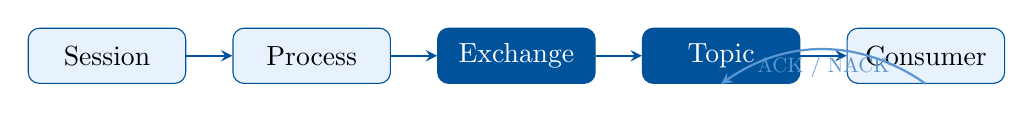
\begin{tikzpicture}[>=stealth]
      \node[draw=SGBlue,fill=SGLightBlue,rounded corners,minimum width=2.0cm,minimum height=.7cm] (session) at (0,0) {Session};
      \node[draw=SGBlue,fill=SGLightBlue,rounded corners,minimum width=2.0cm,minimum height=.7cm] (proc) at (2.6,0) {Process};
      \node[draw=SGBlue,fill=SGBlue,text=white,rounded corners,minimum width=2.0cm,minimum height=.7cm] (exchange) at (5.2,0) {Exchange};
      \node[draw=SGBlue,fill=SGBlue,text=white,rounded corners,minimum width=2.0cm,minimum height=.7cm] (topic) at (7.8,0) {Topic};
      \node[draw=SGBlue,fill=SGLightBlue,rounded corners,minimum width=2.0cm,minimum height=.7cm] (consumer) at (10.4,0) {Consumer};
      \draw[->,thick,SGBlue] (session) -- (proc);
      \draw[->,thick,SGBlue] (proc) -- (exchange);
      \draw[->,thick,SGBlue] (exchange) -- (topic);
      \draw[->,thick,SGBlue] (topic) -- (consumer);
      \draw[->,thick,SGMidBlue,bend right=35] (consumer.south) to node[below,scale=.75]{ACK / NACK} (topic.south);
    \end{tikzpicture}
  \end{center}
  \vspace{.75em}
  \begin{block}{Central design idea}
    Keep routing in Exchange, keep message lifecycle in Topic, and keep TCP
    ownership in Session. Each boundary communicates through explicit commands.
  \end{block}
\end{frame}

\begin{frame}{Conclusion}
  \begin{itemize}
    \item Socket-Go is an application-layer messaging protocol over TCP.
    \item Custom framing converts a byte stream into logical messages.
    \item Topic actors provide queueing, delivery, ACK, retry, and backpressure.
    \item At-least-once semantics improve recovery but require duplicate tolerance.
    \item The design is ready for separate live demonstration and benchmark discussion.
  \end{itemize}
  \vfill
  \begin{center}
    {\Large\blue{Thank you}}\\[.35em]
    Questions?
  \end{center}
\end{frame}

\end{document}
